% !TeX spellcheck = id_ID
\documentclass[a4paper,12pt]{article}
\usepackage[bahasa]{babel}
\usepackage{graphicx}
\usepackage{multirow}
\usepackage{enumitem}
\usepackage{listings}
\usepackage{wrapfig}
\usepackage[T1]{fontenc}
\usepackage{inconsolata}
\usepackage{lipsum}
\usepackage{adjustbox}


\usepackage{color}
\usepackage[table]{xcolor}
\definecolor{pblue}{rgb}{0.13,0.13,1}
\definecolor{pgreen}{rgb}{0,0.5,0}
\definecolor{pred}{rgb}{0.9,0,0}
\definecolor{pgrey}{rgb}{0.46,0.45,0.48}
\lstset{language=Java,
	showspaces=false,
	showtabs=false,
	breaklines=true,
	showstringspaces=false,
	breakatwhitespace=true,
	commentstyle=\color{pgreen},
	keywordstyle=\color{pblue},
	stringstyle=\color{pred},
	rulecolor=\color{black},
	basicstyle=\ttfamily,
	moredelim=[il][\textcolor{pgrey}]{$$},
	moredelim=[is][\textcolor{pgrey}]{\%\%}{\%\%}
}

\graphicspath{ {./img/} }
\begin{document}
\title{ {\Large Laporan Praktikum}\\ Algoritma dan Pemrograman \\{\Large Pertemuan 10}}

\author{Aldzikri Dwijayanto Prathama 
	\\195410189
	\\Teknik Informatika}
\makeatletter
\begin{titlepage}
	\begin{center}
		{\huge \bfseries \@title }\\[14ex]
		
\includegraphics[scale=.8]{logo}\\[4ex]
		{\large \@author}\\[19ex]
		{\large \bfseries {SEKOLAH TINGGI MANAJEMEN INFORMATIKA DAN KOMPUTER
				AKAKOM YOGYAKARTA}}
	\end{center}


%{\large \@date} 
\end{titlepage}
\makeatother
%\maketitle
\newpage
\tableofcontents
\newpage

\section{Tujuan}
Mahasiswa dapat mengimplementasikan konsep perulangan bertingkat dua untuk
menyelesaikan kasus

\section{Dasar Teori}
\paragraph{}
Perulangan adalah model pengembangan sistem yang bersifat dinamis dalam artian
setiap tahapan proses pengembangan sistem dapat diulang jika terdapat kekurangan
atau kesalahan. Setiap tahapan pengembangan sistem dapat dikerjakan berupa
ringkasan dan tidak lengkap, namun pada akhir pengembangan akan didapatkan sistem
yang lengkap pada pengembangan sistem.
Di dalam komputer/pemrograman, iterasi adalah sifat tertentu dari algoritma atau
program komputer di mana suatu urutan atau lebih dari langkah algoritmik dilakukan di
loop (perulangan) program.
Perulangan bersarang/bertingkat/nested loop adalah apabila pada blok statement
perulangan terdapat perulangan lagi, jadi dapat dikatakan perulangan di dalam
perulangan. perulangannya bisa 2 atau lebih.
Sebuah program mengizinkan blok pengulangan di dalam blok pengulangan lainnya, dan
tidak membatasai jenis pengulangan apa yang boleh berada di dalam pengulangan
lainnya, misalnya di dalam blok pengulangan for terdapat pengulangan while, atau didalam pengulangan while terdapat pengulangan for

\newpage
\section{Praktik}
\subsection{Praktik 1}
\begin{center}
	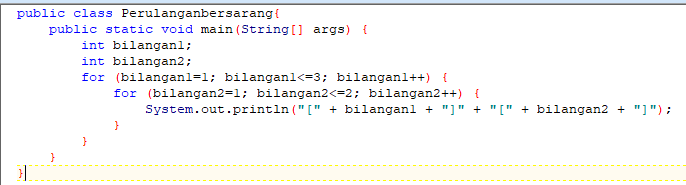
\includegraphics[scale=.7]{Capture1}
\end{center}
pada potongan program diatas terdapa dua for atau perulangan dimana cara kerjanya adalah perulangan for yang berada didalam akan dikerjakan lebih dulu sampai selesai lalu baru dikerjakan for yang luar atau for pertama.\\
Jika program di atas dijalankan maka outputnya seperti berikut.
\begin{center}
	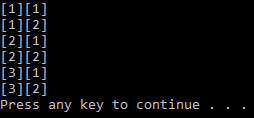
\includegraphics[scale=.7]{Capture2}
\end{center}

\subsection{Praktik 2}
Praktik selanjutnya adalah mengubah perulangan for pada praktik 1, menjadi perulangan while
\begin{center}
	\includegraphics[scale=.7]{capture3}
\end{center}
Jika perulangan for diganti menjadi perulangan while, maka kita harus mendeklarasikan terlebih dahulu variabel yang akan digunakan untuk perulangan. Untuk perulangan kedua, nilai variabel bilangan 2, diletakan didalam perulangan pertama sebelum perulangan kedua, supaya nilai dari variabel yang digunakan oleh perulangan kedua kembali ke nilai awal, jika perulangan kedua selesai dikerjakan.\\
Jika program di atas dijalankan, maka outputnya sama dengan praktik pertama
\begin{center}
	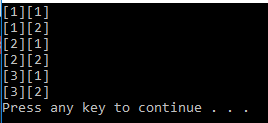
\includegraphics[scale=.7]{Capture4}
\end{center}

\subsection{Praktik 3}

\end{document}